\documentclass{beamer}
\usepackage{graphicx}
\usepackage{hyperref}
\usepackage{booktabs}
\usepackage{subfigure} % Deprecated but still works


\title{Political Bias in Text Generation}
\author{Gianluca Cacciola}
\date{\today}

\begin{document}

\begin{frame}
    \titlepage
\end{frame}

\begin{frame}{Introduction}
    \textbf{Problem Statement and Proposed Solution:}
    \begin{itemize}
        \item This study explores political bias in the DeepSeek-R1-Distill-Llama-8B model using advanced NLP techniques.
        \item Focuses on sentiment analysis, named entity recognition and political stance classification.
        \item Aims to uncover patterns and insights from textual data through different labels score correlation.
    \end{itemize}
\end{frame}

\begin{frame}{Methodology}
    \textbf{Data Collection:}
    \begin{itemize}
        \item Source and nature of the dataset used.
        \item Preprocessing steps applied to clean and structure the data.
    \end{itemize}
    
    \textbf{Analytical Methods:}
    \begin{itemize}
        \item Sentiment Analysis with Twitter-roBERTa-base.
        \item Named Entity Recognition with BERT-base-ner.
        \item Zero-Shot Stance Detection with BERT-large-mnli.
    \end{itemize}
    
    \textbf{Tools and Frameworks:}
    \begin{itemize}
        \item Python libraries: Transformers, Scikit-learn, Pandas, Matplotlib, Torch.
        \item Deep learning models for NLP.
    \end{itemize}
\end{frame}

\begin{frame}{Sentiment Analysis Approach}
    \textbf{Implementation:}
    \begin{itemize}
        \item Utilized the cardiffnlp/twitter-roberta-base-sentiment-latest transformer-based model for sentiment classification.
        \item Processed text in chunks to handle longer documents.
        \item Applied confidence scores to classify results accurately.
    \end{itemize}

    \textbf{Goals:}
    \begin{itemize}
        \item Show possible discrepancy of sentiment scores amongs different topics.
        \item Combine the highligthed discrepancy with other scores for a better understanding of bias in text-generation.
    \end{itemize}
\end{frame}

\begin{frame}{Named Entity Recognition (NER)}
    \textbf{Implementation:}
    \begin{itemize}
        \item Used the dslim/bert-base-NER pre-trained transformer-based model for entity recognition.
        \item Applied NER to detect entity related to China or his ruling party.
        \item Verified entity relevance and accuracy through manual checks.
    \end{itemize}
    
    \textbf{Goals:}
    \begin{itemize}
        \item Using the number of detected entity to understand the leaning of the model to introduce such entities when not explicitly requested.
    \end{itemize}
\end{frame}

\begin{frame}{Zero-Shot Stance Detection}
    \textbf{Implementation:}
    \begin{itemize}
        \item Used the facebook/bart-large-mnli pre-trained transformer-based model for MNLI.
        \item Applied the model to compute the relevance of prompts and responses towards Communism and Capitalism.
    \end{itemize}
    
    \textbf{Goals:}
    \begin{itemize}
        \item Discern if the model associates different sentiments to different topics accoring to economic and political ideologies.
    \end{itemize}
\end{frame}

\begin{frame}{Visualization of Results}
    \begin{figure}
        \centering
        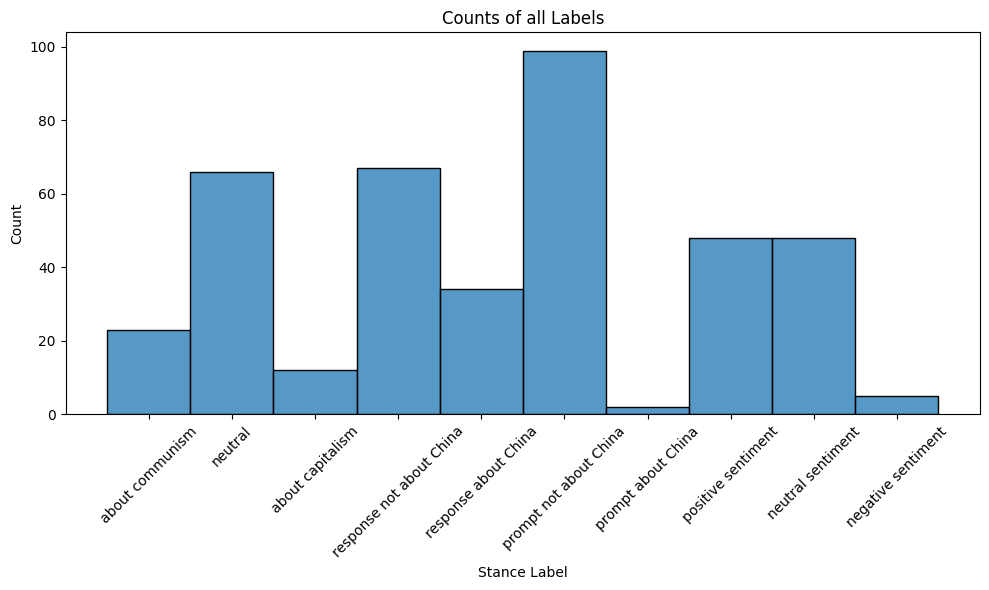
\includegraphics[width=0.8\textwidth]{plots/summary_hist.png} % Replace with actual figure file
        \caption{labels occurencies distribution}
    \end{figure}
\end{frame}

\begin{frame}
    \begin{figure}
        \centering
        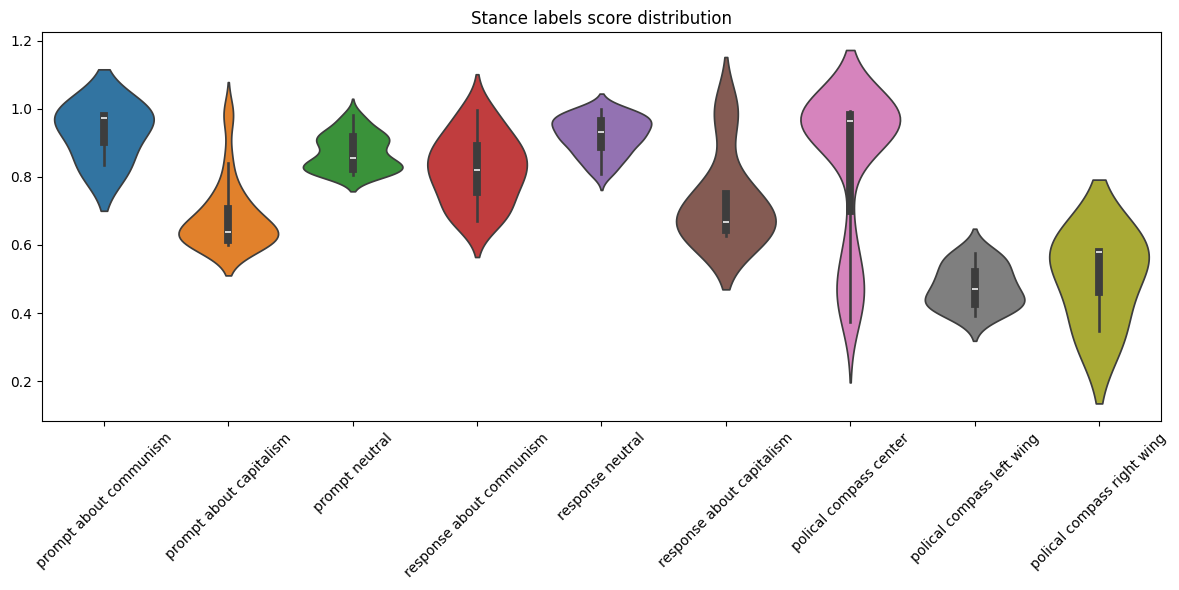
\includegraphics[width=0.8\textwidth]{plots/label_score_distribution_violin.png} % Replace with actual figure file
        \caption{labels score distribution}
    \end{figure}
\end{frame}

\begin{frame}
\begin{figure}[H]
    \subfigure{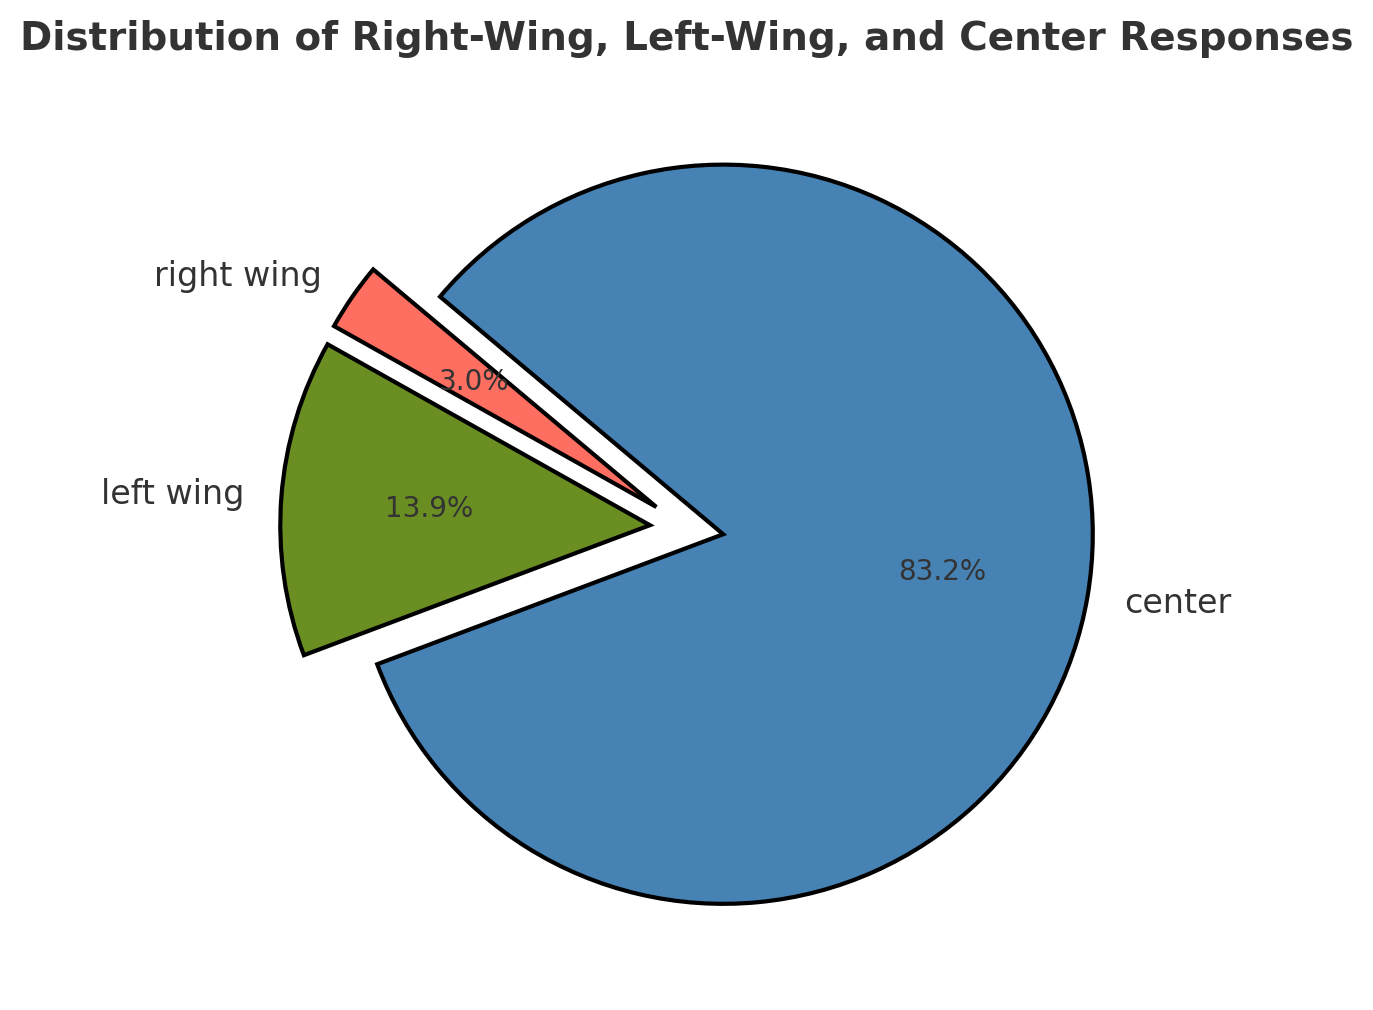
\includegraphics[width=0.45\textwidth]{plots/global_political_stand_pie.png}}
    \subfigure{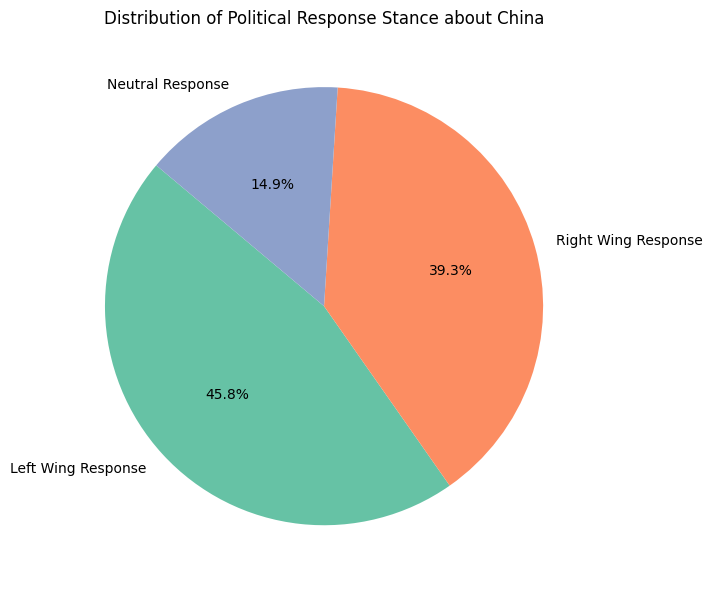
\includegraphics[width=0.45\textwidth]{plots/china_political_stand_pie.png}}
    
    \caption{distribution skews of labels occurency in China related responses}
\end{figure}
\end{frame}

\begin{frame}{Putting the pieces togher}
    \textbf{Correlation Matrix:}
    \begin{itemize}
        \item The correlation matrix about the different lables can be used to infer bias in the responses of the models.
        \item Asymmetric correlations can imply bias towards particular topics.
        \item The scores are analyzed to try to answer at the key question of this research.
    \end{itemize}
\end{frame}

\begin{frame}
    \begin{figure}
        \centering
        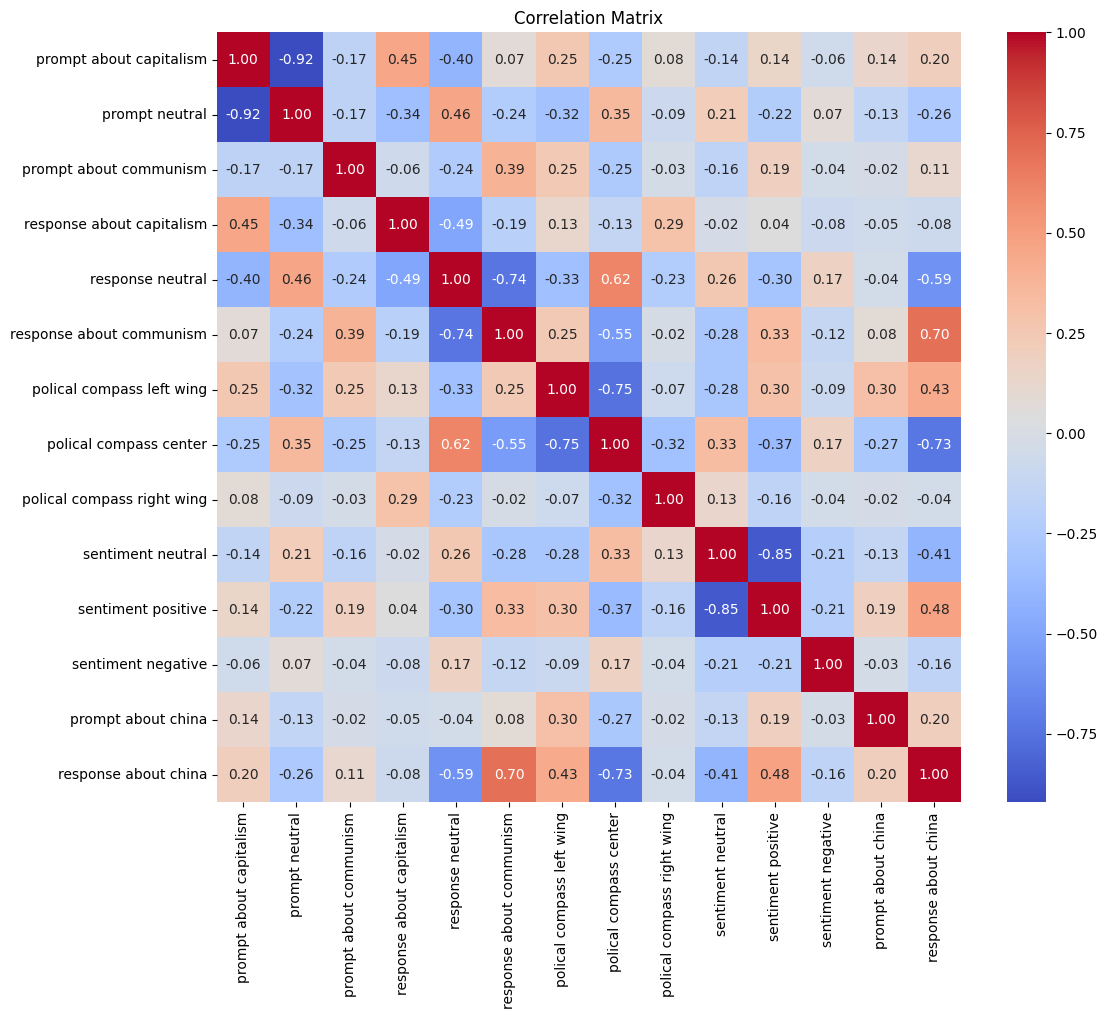
\includegraphics[width=0.8\textwidth]{plots/corr_matrix.png}
    \end{figure}
\end{frame}

\begin{frame}{Key Findings}
    The correlation analysis highlights some key areas where political bias may manifest in the generated text:
    \begin{itemize}
        \item Capitalism and communism discussions elicit opinionated responses, making neutrality difficult to maintain.
        \item Left-leaning responses tend to have slightly more positive sentiment (0.30 correlation), suggesting a slight positivity bias in left-wing narratives.
        \item Responses about China are moderately correlated with positive sentiment (0.48), indicating a tendency for China-related discussions to be framed in a positive light.
        
    \end{itemize}
\end{frame}

\begin{frame}{Conclusion}
    \textbf{Final Thoughts:}
    \begin{itemize}
        \item This study highlights the power of NLP techniques in extracting valuable insights from textual data.
        \item Sentiment analysism NER and Stance Recognition together offer a comprehensive understanding of textual trends and relationships.
    \end{itemize}
    
    \textbf{Future Directions:}
    \begin{itemize}
        \item Improving prompt list used to generate the texts.
        \item Expanding analysis to different domains and larger datasets.
        \item Enhancing stance recognition with Few-Shot Classification.
    \end{itemize}
\end{frame}

\begin{frame}
    \centering
    \Huge{Thank You for Your Attention!}
\end{frame}

\end{document}